\documentclass[11pt,aspectratio=169]{beamer}
\usetheme{Madrid}

% ======================= PACKAGES =======================
\usepackage{graphicx}
\usepackage{booktabs}
\usepackage{adjustbox}
\usepackage{multicol}
\usepackage{amsmath}
\usepackage{amssymb}
\usepackage{tikz}
\usetikzlibrary{arrows,shapes,positioning,shadows,trees}
\usepackage{listings}
\usepackage{xcolor}

% ======================= COLOR DEFINITIONS =======================
% Primary color scheme: Blue/Teal for Digital Finance
\definecolor{dfblue}{RGB}{0,102,204}
\definecolor{dfteal}{RGB}{0,153,153}
\definecolor{dfcyan}{RGB}{51,187,204}
\definecolor{dflightblue}{RGB}{153,204,255}
\definecolor{dflightblue2}{RGB}{173,214,255}
\definecolor{dflightblue3}{RGB}{193,224,255}
\definecolor{dflightblue4}{RGB}{213,234,255}

% Accent colors for finance applications
\definecolor{dfgreen}{RGB}{44, 160, 44}
\definecolor{dfred}{RGB}{214, 39, 40}
\definecolor{dforange}{RGB}{255, 127, 14}
\definecolor{dfgray}{RGB}{127, 127, 127}

% Utility colors
\definecolor{lightgray}{RGB}{240, 240, 240}
\definecolor{midgray}{RGB}{180, 180, 180}
\definecolor{codebg}{RGB}{245, 245, 245}

% ======================= THEME CUSTOMIZATION =======================
% Apply Digital Finance color scheme to Madrid theme
\setbeamercolor{palette primary}{bg=dflightblue3,fg=dfblue}
\setbeamercolor{palette secondary}{bg=dflightblue2,fg=dfblue}
\setbeamercolor{palette tertiary}{bg=dfteal,fg=white}
\setbeamercolor{palette quaternary}{bg=dfblue,fg=white}

\setbeamercolor{structure}{fg=dfblue}
\setbeamercolor{section in toc}{fg=dfblue}
\setbeamercolor{subsection in toc}{fg=dfteal}
\setbeamercolor{title}{fg=dfblue}
\setbeamercolor{frametitle}{fg=dfblue,bg=dflightblue3}
\setbeamercolor{block title}{bg=dflightblue2,fg=dfblue}
\setbeamercolor{block body}{bg=dflightblue4,fg=black}

% Remove navigation symbols for cleaner look
\setbeamertemplate{navigation symbols}{}

% Clean itemize/enumerate
\setbeamertemplate{itemize items}[circle]
\setbeamertemplate{enumerate items}[default]

% Margins for readability
\setbeamersize{text margin left=8mm,text margin right=8mm}

% ======================= LISTINGS CONFIGURATION =======================
% Python code style
\lstdefinestyle{pythonstyle}{
    language=Python,
    basicstyle=\ttfamily\footnotesize,
    keywordstyle=\color{dfblue}\bfseries,
    stringstyle=\color{dforange},
    commentstyle=\color{dfgray}\itshape,
    numberstyle=\tiny\color{dfgray},
    numbers=left,
    numbersep=5pt,
    backgroundcolor=\color{codebg},
    showspaces=false,
    showstringspaces=false,
    showtabs=false,
    frame=single,
    rulecolor=\color{midgray},
    tabsize=4,
    captionpos=b,
    breaklines=true,
    breakatwhitespace=false,
    escapeinside={(*@}{@*)},
    xleftmargin=10pt,
    xrightmargin=10pt
}

% Solidity code style
\lstdefinestyle{soliditystyle}{
    language=Java, % closest approximation
    basicstyle=\ttfamily\footnotesize,
    keywordstyle=\color{dfteal}\bfseries,
    stringstyle=\color{dforange},
    commentstyle=\color{dfgray}\itshape,
    numberstyle=\tiny\color{dfgray},
    numbers=left,
    numbersep=5pt,
    backgroundcolor=\color{codebg},
    showspaces=false,
    showstringspaces=false,
    showtabs=false,
    frame=single,
    rulecolor=\color{midgray},
    tabsize=2,
    captionpos=b,
    breaklines=true,
    breakatwhitespace=false,
    escapeinside={(*@}{@*)},
    xleftmargin=10pt,
    xrightmargin=10pt,
    morekeywords={pragma, contract, function, returns, public, private, view, pure, payable, address, uint256, mapping, event, modifier}
}

% Inline code command
\newcommand{\code}[1]{\texttt{\color{dfblue}#1}}

% ======================= CUSTOM COMMANDS =======================
% Bottom annotation (Madrid-style)
\newcommand{\bottomnote}[1]{%
\vfill
\vspace{-2mm}
\textcolor{dflightblue2}{\rule{\textwidth}{0.4pt}}
\vspace{1mm}
\footnotesize
\textbf{#1}
}

% Compact list spacing
\newcommand{\compactlist}{%
\setlength{\itemsep}{0pt}%
\setlength{\parskip}{0pt}%
\setlength{\parsep}{0pt}%
}

% Chart placeholder
\newcommand{\chartplaceholder}[2][5cm]{%
\begin{center}
\begin{adjustbox}{max width=0.95\textwidth, max height=#1}
\framebox[\textwidth][c]{%
\rule{0pt}{#1}%
\textcolor{midgray}{[#2]}%
}
\end{adjustbox}
\end{center}
}

% ======================= FINANCE NOTATION MACROS =======================
% Probability and statistics
\newcommand{\E}{\mathbb{E}} % Expected value
\newcommand{\Var}{\mathrm{Var}} % Variance
\newcommand{\Cov}{\mathrm{Cov}} % Covariance
\newcommand{\Prob}{\mathbb{P}} % Probability

% Distributions
\newcommand{\Normal}{\mathcal{N}} % Normal distribution
\newcommand{\Uniform}{\mathcal{U}} % Uniform distribution

% Returns and prices
\newcommand{\Ret}{R} % Return
\newcommand{\LogRet}{r} % Log return
\newcommand{\Price}{S} % Price/Stock price
\newcommand{\Strike}{K} % Strike price

% Options and derivatives
\newcommand{\CallPrice}{C} % Call option price
\newcommand{\PutPrice}{P} % Put option price
\newcommand{\Greeks}[1]{\mathit{#1}} % Greek letters

% Risk measures
\newcommand{\VaR}{\mathrm{VaR}} % Value at Risk
\newcommand{\CVaR}{\mathrm{CVaR}} % Conditional VaR
\newcommand{\Sharpe}{\mathrm{SR}} % Sharpe Ratio

% Time series
\newcommand{\AR}{\mathrm{AR}} % Autoregressive
\newcommand{\MA}{\mathrm{MA}} % Moving average
\newcommand{\GARCH}{\mathrm{GARCH}} % GARCH

% Blockchain/Crypto
\newcommand{\Hash}{\mathrm{Hash}} % Hash function
\newcommand{\Block}{\mathcal{B}} % Block
\newcommand{\Chain}{\mathcal{C}} % Chain

% Real numbers, integers
\newcommand{\R}{\mathbb{R}}
\newcommand{\Z}{\mathbb{Z}}
\newcommand{\N}{\mathbb{N}}

% ======================= TIKZ STYLES =======================
% Styles for finance-related diagrams
\tikzstyle{process} = [rectangle, minimum width=3cm, minimum height=1cm, text centered, draw=dfblue, fill=dflightblue4, thick]
\tikzstyle{decision} = [diamond, minimum width=3cm, minimum height=1cm, text centered, draw=dfteal, fill=dflightblue4, thick]
\tikzstyle{arrow} = [thick,->,>=stealth,color=dfblue]
\tikzstyle{blockchain} = [rectangle, rounded corners, minimum width=2.5cm, minimum height=1cm, text centered, draw=dfteal, fill=dflightblue3, thick]
\tikzstyle{transaction} = [circle, minimum size=0.8cm, text centered, draw=dforange, fill=dflightblue4, thick]

% ======================= FOOTER TEMPLATE =======================
\setbeamertemplate{footline}{
    \hbox{\begin{beamercolorbox}[wd=\paperwidth,ht=2.5ex,dp=1ex,leftskip=.5em,rightskip=.5em]{author in head/foot}
    \tiny
    \textbf{Digital Finance} \hfill
    Joerg Osterrieder \hfill
    \insertdate \hfill
    Page \insertframenumber{} / \inserttotalframenumber
    \end{beamercolorbox}}
}

% ======================= SECTION DIVIDER TEMPLATE =======================
\AtBeginSection[]{
\begin{frame}[plain]
\vfill
\centering
\begin{beamercolorbox}[sep=12pt,center]{title}
\usebeamerfont{title}\LARGE\insertsection\par
\end{beamercolorbox}
\vfill
\end{frame}
}


% Document Information
\title[Topic 5.2]{Topic 5.2: Regulatory Landscapes}
\subtitle{Global Approaches to Digital Finance Regulation}
\author{Joerg Osterrieder}
\institute{Digital Finance}
\date{2025}

\begin{document}

% ==============================================================================
% SLIDE 1: Title Slide
% ==============================================================================
\begin{frame}[plain]
\titlepage
\end{frame}

% ==============================================================================
% SLIDE 2: Learning Objectives
% ==============================================================================
\begin{frame}{Learning Objectives}
\textbf{By the end of this topic, you will be able to:}
\vspace{3mm}

\begin{enumerate}
\item \textbf{Compare} major regulatory frameworks across jurisdictions (US, EU, Asia)
\item \textbf{Explain} the policy rationale behind key digital finance regulations
\item \textbf{Apply} the Howey Test to determine security classification of tokens
\item \textbf{Analyze} how regulation shapes innovation trajectories in different markets
\item \textbf{Understand} why identical technology receives different regulatory treatment
\item \textbf{Evaluate} trade-offs between consumer protection and innovation
\end{enumerate}

\vspace{3mm}
\begin{block}{Core Skill}
Regulatory analysis is essential for any digital finance professional---whether building products, investing, or advising clients.
\end{block}
\end{frame}

% ==============================================================================
% SLIDE 3: Prerequisites/Background I
% ==============================================================================
\begin{frame}{Prerequisites: Financial Regulation Basics}
\textbf{Why do we regulate financial markets?}
\vspace{3mm}

\begin{columns}[T]
\begin{column}{0.48\textwidth}
\textbf{Market Failures Addressed:}
\begin{itemize}
\item \textbf{Information asymmetry}---issuers know more than investors
\item \textbf{Systemic risk}---interconnected failures cascade
\item \textbf{Externalities}---fraud harms market confidence
\item \textbf{Public goods}---market integrity benefits all
\end{itemize}
\end{column}
\begin{column}{0.48\textwidth}
\textbf{Core Regulatory Goals:}
\begin{itemize}
\item Consumer/investor protection
\item Market integrity and fairness
\item Financial system stability
\item Prevention of illicit finance
\item Capital formation efficiency
\end{itemize}
\end{column}
\end{columns}

\vspace{5mm}
\begin{alertblock}{The Challenge}
Digital finance challenges traditional regulatory assumptions: borderless, pseudonymous, automated, and often decentralized.
\end{alertblock}
\end{frame}

% ==============================================================================
% SLIDE 4: Prerequisites/Background II
% ==============================================================================
\begin{frame}{Prerequisites: Key Regulatory Concepts}
\begin{center}
\renewcommand{\arraystretch}{1.4}
\begin{tabular}{|l|p{8cm}|}
\hline
\textbf{Concept} & \textbf{Definition} \\
\hline
\textbf{Securities regulation} & Rules governing investment contracts, requiring disclosure and registration \\
\hline
\textbf{AML/KYC} & Anti-Money Laundering / Know Your Customer---identity verification and transaction monitoring \\
\hline
\textbf{Money transmission} & Transferring funds on behalf of others---requires licensing \\
\hline
\textbf{Prudential regulation} & Rules ensuring financial institutions remain solvent \\
\hline
\textbf{Consumer protection} & Safeguards against fraud, manipulation, unfair practices \\
\hline
\textbf{Regulatory arbitrage} & Choosing favorable jurisdictions to minimize compliance \\
\hline
\end{tabular}
\end{center}

\vspace{3mm}
\textbf{Key insight:} The same crypto activity may trigger multiple regulatory regimes simultaneously.
\end{frame}

% ==============================================================================
% SLIDE 5: The Regulatory Challenge
% ==============================================================================
\begin{frame}{The Regulatory Challenge}
\begin{columns}[T]
\begin{column}{0.48\textwidth}
\textbf{What regulators want:}
\begin{itemize}
\item Consumer protection
\item Market integrity
\item Financial stability
\item Anti-money laundering
\item Tax compliance
\item National security
\end{itemize}
\end{column}
\begin{column}{0.48\textwidth}
\textbf{What innovators want:}
\begin{itemize}
\item Permissionless access
\item Privacy
\item Speed to market
\item Global reach
\item Minimal compliance costs
\item Regulatory clarity
\end{itemize}
\end{column}
\end{columns}

\vspace{5mm}
\begin{center}
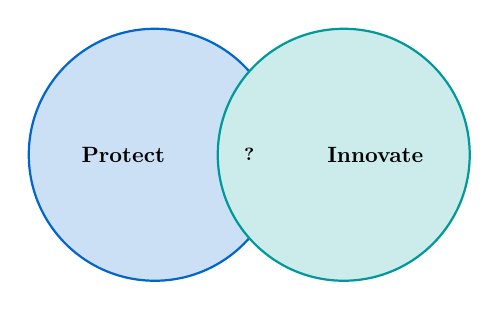
\begin{tikzpicture}[scale=0.8, transform shape]
\draw[thick, dfblue, fill=dfblue!20] (0,0) circle (2cm);
\draw[thick, dfteal, fill=dfteal!20] (3,0) circle (2cm);

\node at (-0.5,0) {\textbf{Protect}};
\node at (3.5,0) {\textbf{Innovate}};
\node at (1.5,0) {\footnotesize \textbf{?}};
\end{tikzpicture}
\end{center}
\end{frame}

% ==============================================================================
% SLIDE 6: US Fragmented Landscape
% ==============================================================================
\begin{frame}{United States: Fragmented Regulatory Landscape}
\begin{center}
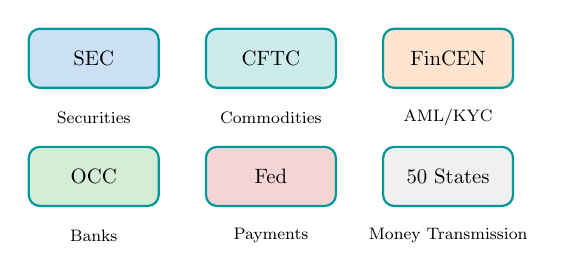
\begin{tikzpicture}[scale=0.75, transform shape]
% Regulatory agencies
\node (sec) [blockchain, minimum width=2.2cm, fill=dfblue!20] {SEC};
\node (cftc) [blockchain, right of=sec, node distance=3cm, minimum width=2.2cm, fill=dfteal!20] {CFTC};
\node (fincen) [blockchain, right of=cftc, node distance=3cm, minimum width=2.2cm, fill=dforange!20] {FinCEN};
\node (occ) [blockchain, below of=sec, node distance=2cm, minimum width=2.2cm, fill=dfgreen!20] {OCC};
\node (fed) [blockchain, below of=cftc, node distance=2cm, minimum width=2.2cm, fill=dfred!20] {Fed};
\node (state) [blockchain, below of=fincen, node distance=2cm, minimum width=2.2cm, fill=lightgray] {50 States};

% Labels
\node[below of=sec, node distance=1cm, font=\footnotesize] {Securities};
\node[below of=cftc, node distance=1cm, font=\footnotesize] {Commodities};
\node[below of=fincen, node distance=1cm, font=\footnotesize] {AML/KYC};
\node[below of=occ, node distance=1cm, font=\footnotesize] {Banks};
\node[below of=fed, node distance=1cm, font=\footnotesize] {Payments};
\node[below of=state, node distance=1cm, font=\footnotesize] {Money Transmission};
\end{tikzpicture}
\end{center}

\vspace{3mm}
\begin{alertblock}{Key Issue}
No single regulator for crypto. Jurisdictional conflicts between SEC (securities) and CFTC (commodities) create uncertainty and ``regulation by enforcement.''
\end{alertblock}
\end{frame}

% ==============================================================================
% SLIDE 7: The Howey Test
% ==============================================================================
\begin{frame}{US: The Howey Test}
\begin{columns}[T]
\begin{column}{0.55\textwidth}
\textbf{Is it a security?}\\
A token is a security if it involves:
\begin{enumerate}
\item \textbf{Investment of money}
\item \textbf{In a common enterprise}
\item \textbf{With expectation of profits}
\item \textbf{Derived from others' efforts}
\end{enumerate}

\vspace{3mm}
\textbf{SEC Position:}
\begin{itemize}
\item Most ICOs were securities
\item Many tokens are securities
\item ETH and BTC are NOT securities
\item ``Come in and register''
\end{itemize}
\end{column}
\begin{column}{0.42\textwidth}
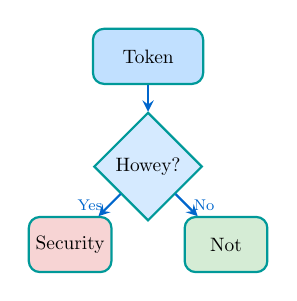
\begin{tikzpicture}[scale=0.7, transform shape]
% Decision tree
\node (start) [blockchain, minimum width=2cm] {Token};
\node (howey) [decision, below of=start, node distance=2cm, minimum width=1.5cm, minimum height=1.5cm] {Howey?};
\node (security) [blockchain, below left of=howey, node distance=2cm, fill=dfred!20, minimum width=1.5cm] {Security};
\node (commodity) [blockchain, below right of=howey, node distance=2cm, fill=dfgreen!20, minimum width=1.5cm] {Not};

\draw[arrow] (start) -- (howey);
\draw[arrow] (howey) -- node[left, font=\footnotesize] {Yes} (security);
\draw[arrow] (howey) -- node[right, font=\footnotesize] {No} (commodity);
\end{tikzpicture}

\vspace{3mm}
\textbf{Consequences:}\\
\footnotesize Securities require registration, prospectus, qualified investors only.
\end{column}
\end{columns}
\end{frame}

% ==============================================================================
% SLIDE 8: SEC vs CFTC Jurisdiction
% ==============================================================================
\begin{frame}{SEC vs. CFTC: Jurisdictional Divide}
\begin{center}
\renewcommand{\arraystretch}{1.3}
\begin{tabular}{|l|c|c|}
\hline
\textbf{Aspect} & \textbf{SEC} & \textbf{CFTC} \\
\hline
\textbf{Jurisdiction} & Securities & Commodities \\
\hline
\textbf{Key test} & Howey Test & Not a security \\
\hline
\textbf{Bitcoin} & Not a security & Commodity \\
\hline
\textbf{Ethereum} & Not a security (debated) & Commodity \\
\hline
\textbf{Most altcoins} & Often securities & Spot market limited \\
\hline
\textbf{Stablecoins} & Unclear & Limited jurisdiction \\
\hline
\textbf{Exchanges} & Securities exchanges & Derivatives exchanges \\
\hline
\end{tabular}
\end{center}

\vspace{3mm}
\begin{block}{The Gap}
Spot markets for crypto commodities (like Bitcoin) fall into a regulatory gap---CFTC has limited authority, SEC claims none.
\end{block}
\end{frame}

% ==============================================================================
% SLIDE 9: FinCEN and AML Requirements
% ==============================================================================
\begin{frame}{FinCEN: AML/KYC Requirements}
\textbf{Financial Crimes Enforcement Network (FinCEN)}---enforces Bank Secrecy Act
\vspace{3mm}

\begin{columns}[T]
\begin{column}{0.48\textwidth}
\textbf{Who must register?}
\begin{itemize}
\item Crypto exchanges
\item Custodial wallet providers
\item Crypto ATM operators
\item Payment processors
\item (As Money Services Businesses)
\end{itemize}
\end{column}
\begin{column}{0.48\textwidth}
\textbf{Requirements:}
\begin{itemize}
\item Customer identification (KYC)
\item Transaction monitoring
\item Suspicious Activity Reports (SARs)
\item Currency Transaction Reports (\$10K+)
\item Record keeping (5 years)
\end{itemize}
\end{column}
\end{columns}

\vspace{5mm}
\begin{alertblock}{Key Point}
AML/KYC requirements apply regardless of whether tokens are securities or commodities. All crypto businesses touching fiat or custody must comply.
\end{alertblock}
\end{frame}

% ==============================================================================
% SLIDE 10: US Enforcement Actions
% ==============================================================================
\begin{frame}{US Enforcement Actions (2023-2024)}
\begin{center}
\renewcommand{\arraystretch}{1.3}
\begin{tabular}{|l|l|p{5cm}|}
\hline
\textbf{Target} & \textbf{Allegation} & \textbf{Status} \\
\hline
Coinbase & Operating unregistered exchange & Ongoing litigation \\
\hline
Binance & Multiple securities violations & \$4.3B settlement \\
\hline
Kraken & Unregistered staking service & \$30M settlement \\
\hline
Ripple (XRP) & Unregistered securities & Partial win for Ripple \\
\hline
Terraform & Securities fraud (UST) & Founders charged \\
\hline
\end{tabular}
\end{center}

\vspace{3mm}
\begin{alertblock}{Regulation by Enforcement}
The US lacks comprehensive crypto legislation. SEC and CFTC establish rules through lawsuits rather than clear guidelines.
\end{alertblock}
\end{frame}

% ==============================================================================
% SLIDE 11: State-Level Regulation
% ==============================================================================
\begin{frame}{US State-Level Regulation: BitLicense Example}
\textbf{New York BitLicense (2015)}---most comprehensive state framework
\vspace{3mm}

\begin{columns}[T]
\begin{column}{0.48\textwidth}
\textbf{Requirements:}
\begin{itemize}
\item Application fee + capital reserves
\item Comprehensive cybersecurity program
\item AML/KYC compliance plan
\item Consumer protection measures
\item Books and records requirements
\item Regular examinations
\end{itemize}
\end{column}
\begin{column}{0.48\textwidth}
\textbf{Impact:}
\begin{itemize}
\item Many companies exit NY market
\item High compliance costs
\item Lengthy approval process
\item But: regulatory clarity
\item Other states: Wyoming (friendly), Texas (mixed)
\end{itemize}
\end{column}
\end{columns}

\vspace{3mm}
\begin{block}{50-State Problem}
Each US state has different money transmission rules. Operating nationally requires up to 50 separate licenses.
\end{block}
\end{frame}

% ==============================================================================
% SLIDE 12: Securities Exemptions
% ==============================================================================
\begin{frame}{US: Securities Registration Exemptions}
\textbf{If your token is a security, how can you legally issue it?}
\vspace{3mm}

\begin{center}
\renewcommand{\arraystretch}{1.3}
\footnotesize
\begin{tabular}{|l|p{3.5cm}|p{4cm}|p{2.5cm}|}
\hline
\textbf{Exemption} & \textbf{What It Allows} & \textbf{Key Requirements} & \textbf{Investor Limits} \\
\hline
\textbf{Reg D 506(b)} & Private placement & No general solicitation & Accredited only \\
\hline
\textbf{Reg D 506(c)} & Private placement & Can advertise, verify status & Accredited only \\
\hline
\textbf{Reg A+} & Mini-IPO up to \$75M & Light SEC review, ongoing disclosure & Anyone (with limits) \\
\hline
\textbf{Reg S} & Non-US offering & Offshore only, no US marketing & Non-US persons \\
\hline
\textbf{Reg CF} & Crowdfunding up to \$5M & Through registered portal & Anyone (with limits) \\
\hline
\end{tabular}
\end{center}

\vspace{3mm}
\textbf{Warning:} Exemptions have strict requirements. Violations trigger enforcement.
\end{frame}

% ==============================================================================
% SLIDE 13: EU MiCA Framework
% ==============================================================================
\begin{frame}{European Union: MiCA Framework}
\begin{columns}[T]
\begin{column}{0.55\textwidth}
\textbf{Markets in Crypto-Assets (MiCA):}
\begin{itemize}
\item First comprehensive crypto regulation
\item Effective 2024-2025
\item Harmonized across 27 countries
\item Clear licensing requirements
\end{itemize}

\vspace{3mm}
\textbf{Key Provisions:}
\begin{enumerate}
\item Crypto-Asset Service Providers (CASPs) licensed
\item Stablecoin issuers must hold reserves
\item Whitepaper requirements for token issuance
\item Consumer protection rules
\item Market manipulation prohibited
\end{enumerate}
\end{column}
\begin{column}{0.42\textwidth}
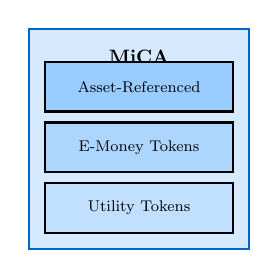
\begin{tikzpicture}[scale=0.7, transform shape]
% MiCA structure
\draw[thick, dfblue, fill=dflightblue4] (0,0) rectangle (4,4);
\node at (2,3.5) {\textbf{MiCA}};

\draw[thick, fill=dflightblue3] (0.3,0.3) rectangle (3.7,1.2);
\node[font=\footnotesize] at (2,0.75) {Utility Tokens};

\draw[thick, fill=dflightblue2] (0.3,1.4) rectangle (3.7,2.3);
\node[font=\footnotesize] at (2,1.85) {E-Money Tokens};

\draw[thick, fill=dflightblue] (0.3,2.5) rectangle (3.7,3.4);
\node[font=\footnotesize] at (2,2.95) {Asset-Referenced};
\end{tikzpicture}

\vspace{3mm}
\footnotesize
\textbf{Not covered:}\\
DeFi, NFTs (mostly), CBDCs
\end{column}
\end{columns}
\end{frame}

% ==============================================================================
% SLIDE 14: MiCA Token Categories
% ==============================================================================
\begin{frame}{MiCA: Token Categories}
\begin{center}
\renewcommand{\arraystretch}{1.4}
\footnotesize
\begin{tabular}{|l|p{4cm}|p{5cm}|}
\hline
\textbf{Category} & \textbf{Definition} & \textbf{Requirements} \\
\hline
\textbf{Utility Tokens} & Provide access to goods/services on a platform & Whitepaper, fair marketing, basic disclosure \\
\hline
\textbf{Asset-Referenced Tokens (ARTs)} & Value references multiple assets, commodities, or currencies & Authorization, reserve requirements, no interest payments \\
\hline
\textbf{E-Money Tokens (EMTs)} & Pegged 1:1 to single fiat currency & E-money institution license, 1:1 redemption, segregated reserves \\
\hline
\textbf{Other crypto-assets} & BTC, ETH, and similar & Lighter touch, no issuer requirements \\
\hline
\end{tabular}
\end{center}

\vspace{3mm}
\begin{block}{Key Distinction}
MiCA creates clear categories with proportionate requirements---unlike the US binary security/commodity debate.
\end{block}
\end{frame}

% ==============================================================================
% SLIDE 15: MiCA Stablecoin Rules
% ==============================================================================
\begin{frame}{MiCA: Stablecoin Rules}
\begin{columns}[T]
\begin{column}{0.48\textwidth}
\textbf{Asset-Referenced Tokens (ARTs):}
\begin{itemize}
\item Backed by multiple assets
\item Issuer must be authorized
\item Reserve requirements
\item No interest payments
\item If ``significant'': stricter rules
\end{itemize}

\vspace{3mm}
\textbf{E-Money Tokens (EMTs):}
\begin{itemize}
\item Single fiat currency reference
\item Must be e-money institution
\item 1:1 redemption rights
\item Segregated reserves
\end{itemize}
\end{column}
\begin{column}{0.48\textwidth}
\begin{alertblock}{Significance Thresholds}
``Significant'' ART/EMT if:
\begin{itemize}
\item 10M+ holders
\item \EUR{}5B+ market cap
\item 2.5M+ daily transactions
\item \EUR{}500M+ daily value
\end{itemize}
Higher capital, stricter oversight.
\end{alertblock}

\vspace{3mm}
\textbf{Impact on USDT/USDC:}\\
Must comply or delist from EU exchanges.
\end{column}
\end{columns}
\end{frame}

% ==============================================================================
% SLIDE 16: MiCA Service Provider Rules
% ==============================================================================
\begin{frame}{MiCA: Crypto-Asset Service Providers (CASPs)}
\textbf{Services requiring CASP license:}
\vspace{2mm}

\begin{multicols}{2}
\begin{itemize}
\item Custody and administration
\item Operating a trading platform
\item Exchange of crypto for fiat
\item Exchange of crypto for crypto
\item Execution of orders
\item Placing of crypto-assets
\item Transfer services
\item Advice on crypto-assets
\item Portfolio management
\end{itemize}
\end{multicols}

\vspace{3mm}
\textbf{CASP Requirements:}
\begin{itemize}
\item Authorization in one EU member state (passportable)
\item Minimum capital requirements
\item Governance and organizational requirements
\item Safeguarding of client assets
\item Complaints handling procedures
\end{itemize}

\vspace{3mm}
\begin{block}{Passporting}
Once licensed in one EU country, CASPs can operate across all 27 member states.
\end{block}
\end{frame}

% ==============================================================================
% SLIDE 17: Asia Diverse Approaches
% ==============================================================================
\begin{frame}{Asia: Diverse Regulatory Approaches}
\begin{center}
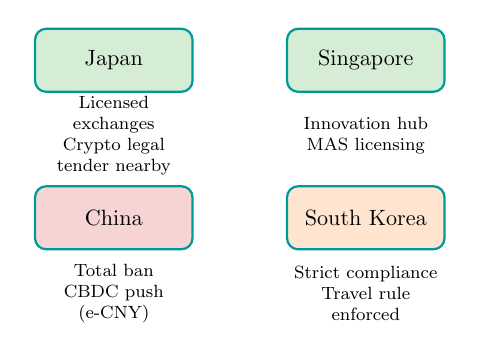
\begin{tikzpicture}[scale=0.8, transform shape]
% Map representation
\node (japan) [blockchain, minimum width=2.5cm, fill=dfgreen!20] {Japan};
\node (singapore) [blockchain, right of=japan, node distance=4cm, minimum width=2.5cm, fill=dfgreen!20] {Singapore};
\node (china) [blockchain, below of=japan, node distance=2.5cm, minimum width=2.5cm, fill=dfred!20] {China};
\node (korea) [blockchain, below of=singapore, node distance=2.5cm, minimum width=2.5cm, fill=dforange!20] {South Korea};

% Labels
\node[below of=japan, node distance=1.2cm, font=\footnotesize, text width=2.5cm, align=center] {Licensed exchanges\\Crypto legal tender nearby};
\node[below of=singapore, node distance=1.2cm, font=\footnotesize, text width=2.5cm, align=center] {Innovation hub\\MAS licensing};
\node[below of=china, node distance=1.2cm, font=\footnotesize, text width=2.5cm, align=center] {Total ban\\CBDC push (e-CNY)};
\node[below of=korea, node distance=1.2cm, font=\footnotesize, text width=2.5cm, align=center] {Strict compliance\\Travel rule enforced};
\end{tikzpicture}
\end{center}

\vspace{3mm}
\textbf{Key insight:} Asia demonstrates the full spectrum from complete ban (China) to innovation hub (Singapore).
\end{frame}

% ==============================================================================
% SLIDE 18: Singapore MAS
% ==============================================================================
\begin{frame}{Singapore: Innovation Hub with Clear Rules}
\textbf{Monetary Authority of Singapore (MAS) Approach}
\vspace{3mm}

\begin{columns}[T]
\begin{column}{0.48\textwidth}
\textbf{Regulatory Framework:}
\begin{itemize}
\item Payment Services Act (PSA) 2019
\item Digital Payment Token (DPT) license
\item Clear licensing categories
\item Risk-based supervision
\item Regulatory sandbox available
\end{itemize}
\end{column}
\begin{column}{0.48\textwidth}
\textbf{Requirements:}
\begin{itemize}
\item AML/CFT compliance
\item Technology risk management
\item User protection measures
\item Capital requirements
\item Fit and proper management
\end{itemize}
\end{column}
\end{columns}

\vspace{5mm}
\begin{block}{Singapore's Strategy}
Attract compliant crypto businesses with clear rules, strict enforcement, and innovation support---while banning retail crypto advertising.
\end{block}
\end{frame}

% ==============================================================================
% SLIDE 19: China Complete Ban
% ==============================================================================
\begin{frame}{China: Complete Ban + CBDC}
\begin{columns}[T]
\begin{column}{0.48\textwidth}
\textbf{What's Banned:}
\begin{itemize}
\item Cryptocurrency trading
\item Crypto mining (since 2021)
\item ICOs
\item Crypto exchanges
\item Providing crypto services
\end{itemize}

\vspace{3mm}
\textbf{Penalties:}
\begin{itemize}
\item Criminal prosecution possible
\item Businesses shut down
\item Mining operations seized
\end{itemize}
\end{column}
\begin{column}{0.48\textwidth}
\textbf{Digital Yuan (e-CNY):}
\begin{itemize}
\item Central Bank Digital Currency
\item Controlled by PBoC
\item Two-tier distribution
\item Programmable money
\item Pilot programs in major cities
\end{itemize}

\vspace{3mm}
\begin{alertblock}{The Strategy}
Ban decentralized crypto, promote centralized CBDC. Maximum control, full surveillance.
\end{alertblock}
\end{column}
\end{columns}
\end{frame}

% ==============================================================================
% SLIDE 20: Japan and South Korea
% ==============================================================================
\begin{frame}{Japan and South Korea: Regulated Markets}
\begin{columns}[T]
\begin{column}{0.48\textwidth}
\textbf{Japan (FSA):}
\begin{itemize}
\item First major country to license exchanges (2017)
\item Crypto as ``payment method''
\item Strict exchange requirements
\item Cold wallet mandate
\item Self-regulatory organization (JVCEA)
\item Response to Mt. Gox collapse
\end{itemize}
\end{column}
\begin{column}{0.48\textwidth}
\textbf{South Korea:}
\begin{itemize}
\item Real-name trading accounts
\item Bank partnerships required
\item Strict Travel Rule enforcement
\item Tax on crypto gains
\item Major exchange oversight
\item High retail participation
\end{itemize}
\end{column}
\end{columns}

\vspace{5mm}
\begin{block}{Common Thread}
Both markets experienced major hacks/scandals that drove stricter regulation. Compliance-focused but open to innovation.
\end{block}
\end{frame}

% ==============================================================================
% SLIDE 21: Regulatory Comparison Matrix
% ==============================================================================
\begin{frame}{Regulatory Comparison Matrix}
\begin{center}
\renewcommand{\arraystretch}{1.2}
\footnotesize
\begin{tabular}{|l|c|c|c|c|}
\hline
\textbf{Aspect} & \textbf{US} & \textbf{EU (MiCA)} & \textbf{Singapore} & \textbf{China} \\
\hline
Crypto trading & Varies & Licensed & Licensed & \textcolor{dfred}{Banned} \\
\hline
Token issuance & Case-by-case & Whitepaper & Licensed & \textcolor{dfred}{Banned} \\
\hline
Stablecoins & Unclear & Regulated & Licensed & \textcolor{dfred}{Banned} \\
\hline
DeFi & Unclear & Unclear & Evolving & \textcolor{dfred}{Banned} \\
\hline
NFTs & Unclear & Mostly exempt & Evolving & Gray area \\
\hline
CBDC & Researching & Exploring & Exploring & \textcolor{dfgreen}{Live} \\
\hline
Clarity & \textcolor{dfred}{Low} & \textcolor{dfgreen}{High} & \textcolor{dforange}{Medium} & \textcolor{dfgreen}{High (ban)} \\
\hline
\end{tabular}
\end{center}

\vspace{3mm}
\begin{block}{Key Insight}
Regulatory arbitrage is real. Projects choose jurisdictions strategically. Clear rules (even strict ones) often preferred over uncertainty.
\end{block}
\end{frame}

% ==============================================================================
% SLIDE 22: The Travel Rule
% ==============================================================================
\begin{frame}{The Travel Rule (FATF Recommendation 16)}
\begin{columns}[T]
\begin{column}{0.55\textwidth}
\textbf{What is it?}\\
FATF requirement: Virtual Asset Service Providers (VASPs) must share sender/receiver information for transfers above thresholds.

\vspace{3mm}
\textbf{Information Required:}
\begin{itemize}
\item Sender name
\item Sender account number
\item Sender address or ID
\item Beneficiary name
\item Beneficiary account number
\end{itemize}

\vspace{3mm}
\textbf{Thresholds:}
\begin{itemize}
\item US: \$3,000+
\item EU: \EUR{}0 (all transfers!)
\item FATF guidance: \$1,000
\end{itemize}
\end{column}
\begin{column}{0.42\textwidth}
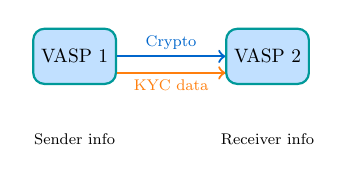
\begin{tikzpicture}[scale=0.7, transform shape, node distance=2cm]
% Travel rule flow
\node (vasp1) [blockchain, minimum width=1.5cm] {VASP 1};
\node (vasp2) [blockchain, right of=vasp1, node distance=3.5cm, minimum width=1.5cm] {VASP 2};

\draw[->, thick, dfblue] (vasp1) -- node[above, font=\footnotesize] {Crypto} (vasp2);
\draw[->, thick, dforange] ([yshift=-3mm]vasp1.east) -- node[below, font=\footnotesize] {KYC data} ([yshift=-3mm]vasp2.west);

\node[below of=vasp1, node distance=1.5cm, font=\footnotesize] {Sender info};
\node[below of=vasp2, node distance=1.5cm, font=\footnotesize] {Receiver info};
\end{tikzpicture}

\vspace{5mm}
\begin{alertblock}{DeFi Challenge}
How do you apply Travel Rule to non-custodial wallets and DEXs?
\end{alertblock}
\end{column}
\end{columns}
\end{frame}

% ==============================================================================
% SLIDE 23: DeFi Regulatory Challenges
% ==============================================================================
\begin{frame}{DeFi Regulatory Challenges}
\begin{columns}[T]
\begin{column}{0.48\textwidth}
\textbf{The Fundamental Problem:}
\begin{itemize}
\item Who is the ``operator''?
\item Where is it located?
\item Who do you regulate?
\item How do you enforce?
\end{itemize}

\vspace{3mm}
\textbf{Potential Targets:}
\begin{itemize}
\item Frontend interfaces
\item Token holders with governance power
\item Core developers
\item Infrastructure providers
\end{itemize}
\end{column}
\begin{column}{0.48\textwidth}
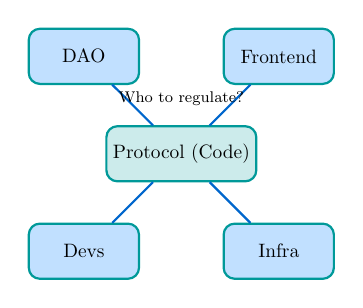
\begin{tikzpicture}[scale=0.7, transform shape]
% DeFi structure
\node (protocol) [blockchain, minimum width=2.5cm, fill=dfteal!20] {Protocol (Code)};
\node (governance) [blockchain, above left of=protocol, node distance=2.5cm, minimum width=2cm] {DAO};
\node (frontend) [blockchain, above right of=protocol, node distance=2.5cm, minimum width=2cm] {Frontend};
\node (devs) [blockchain, below left of=protocol, node distance=2.5cm, minimum width=2cm] {Devs};
\node (infra) [blockchain, below right of=protocol, node distance=2.5cm, minimum width=2cm] {Infra};

\draw[thick, dfblue] (governance) -- (protocol);
\draw[thick, dfblue] (frontend) -- (protocol);
\draw[thick, dfblue] (devs) -- (protocol);
\draw[thick, dfblue] (infra) -- (protocol);

\node[above of=protocol, node distance=1cm, font=\footnotesize] {Who to regulate?};
\end{tikzpicture}
\end{column}
\end{columns}

\vspace{3mm}
\begin{block}{Emerging Approach}
Target the chokepoints: fiat on/off ramps, centralized frontends, infrastructure providers.
\end{block}
\end{frame}

% ==============================================================================
% SLIDE 24: Regulatory Sandbox Concept
% ==============================================================================
\begin{frame}{Regulatory Sandboxes}
\textbf{A controlled environment for innovation under regulatory supervision}
\vspace{3mm}

\begin{columns}[T]
\begin{column}{0.48\textwidth}
\textbf{How Sandboxes Work:}
\begin{enumerate}
\item Company applies with innovative product
\item Regulator grants limited authorization
\item Testing with real users, limited scale
\item Relaxed rules during trial period
\item Evaluation and exit to full compliance
\end{enumerate}
\end{column}
\begin{column}{0.48\textwidth}
\textbf{Countries with Crypto Sandboxes:}
\begin{itemize}
\item UK (FCA)
\item Singapore (MAS)
\item Switzerland (FINMA)
\item UAE (ADGM, DIFC)
\item Bermuda
\item Australia (ASIC)
\end{itemize}
\end{column}
\end{columns}

\vspace{5mm}
\begin{block}{Benefits}
Regulators learn about new technologies. Innovators get clarity. Both sides reduce risk.
\end{block}
\end{frame}

% ==============================================================================
% SLIDE 25: Case Study - Tornado Cash
% ==============================================================================
\begin{frame}{Case Study: Tornado Cash Sanctions}
\begin{columns}[T]
\begin{column}{0.55\textwidth}
\textbf{What Happened (Aug 2022):}
\begin{itemize}
\item US Treasury sanctioned Tornado Cash
\item Smart contract addresses added to OFAC list
\item Developer arrested in Netherlands
\item First time: CODE itself sanctioned
\end{itemize}

\vspace{3mm}
\textbf{Consequences:}
\begin{itemize}
\item GitHub removed repo
\item Circle froze USDC in addresses
\item Exchanges blocked deposits
\item Alchemy/Infura blocked RPC access
\end{itemize}
\end{column}
\begin{column}{0.42\textwidth}
\begin{alertblock}{Legal Questions}
\begin{itemize}
\item Can you sanction open-source code?
\item Is running a mixer illegal?
\item What about privacy rights?
\item First Amendment implications?
\end{itemize}
\end{alertblock}

\vspace{3mm}
\textbf{Outcome:}\\
Court ruled some sanctions overreach (2024). Case ongoing.
\end{column}
\end{columns}
\end{frame}

% ==============================================================================
% SLIDE 26: Case Study - Ripple XRP
% ==============================================================================
\begin{frame}{Case Study: SEC vs. Ripple (XRP)}
\textbf{The landmark case defining token classification}
\vspace{3mm}

\begin{columns}[T]
\begin{column}{0.48\textwidth}
\textbf{SEC's Position:}
\begin{itemize}
\item XRP is a security
\item Ripple raised \$1.3B through unregistered sales
\item Investors expected profits from Ripple's efforts
\item Howey Test clearly applies
\end{itemize}

\vspace{3mm}
\textbf{Timeline:}
\begin{itemize}
\item Dec 2020: SEC files lawsuit
\item July 2023: Summary judgment
\item 2024: Ongoing appeals
\end{itemize}
\end{column}
\begin{column}{0.48\textwidth}
\textbf{July 2023 Ruling:}
\begin{itemize}
\item \textcolor{dfred}{Institutional sales = Securities}
\item \textcolor{dfgreen}{Exchange sales = NOT securities}
\item Programmatic sales to anonymous buyers don't meet Howey
\end{itemize}

\vspace{3mm}
\begin{alertblock}{Implications}
Secondary market trading may not create securities liability. Context matters more than token itself.
\end{alertblock}
\end{column}
\end{columns}
\end{frame}

% ==============================================================================
% SLIDE 27: Case Study - Terra/Luna Collapse
% ==============================================================================
\begin{frame}{Case Study: Terra/Luna Regulatory Aftermath}
\textbf{How regulators respond to \$40B+ collapse}
\vspace{3mm}

\begin{columns}[T]
\begin{column}{0.48\textwidth}
\textbf{What Happened (May 2022):}
\begin{itemize}
\item UST stablecoin de-pegged
\item Algorithmic mechanism failed
\item LUNA dropped 99.99\%
\item \$40B+ market cap destroyed
\item Cascading failures across DeFi
\end{itemize}
\end{column}
\begin{column}{0.48\textwidth}
\textbf{Regulatory Response:}
\begin{itemize}
\item SEC: Securities fraud charges
\item South Korea: Arrest warrants
\item Do Kwon: Arrested in Montenegro
\item MiCA: Influenced stablecoin rules
\item Accelerated global regulation
\end{itemize}
\end{column}
\end{columns}

\vspace{5mm}
\begin{block}{Lesson}
Systemic failures trigger regulatory action. Terra accelerated stablecoin regulation globally, especially in EU (MiCA) and proposed US legislation.
\end{block}
\end{frame}

% ==============================================================================
% SLIDE 28: Case Study - FTX and Exchange Regulation
% ==============================================================================
\begin{frame}{Case Study: FTX Collapse and Exchange Oversight}
\textbf{The case that changed crypto regulation permanently}
\vspace{3mm}

\begin{columns}[T]
\begin{column}{0.48\textwidth}
\textbf{What Failed (Nov 2022):}
\begin{itemize}
\item Customer funds mixed with Alameda
\item No segregation of assets
\item Fraudulent accounting
\item \$8B+ customer funds missing
\item Major contagion effects
\end{itemize}
\end{column}
\begin{column}{0.48\textwidth}
\textbf{Regulatory Implications:}
\begin{itemize}
\item Proof of reserves demanded
\item Customer asset segregation
\item Enhanced disclosure requirements
\item Congressional hearings
\item Accelerated legislation efforts
\end{itemize}
\end{column}
\end{columns}

\vspace{5mm}
\begin{alertblock}{Key Takeaway}
FTX showed that offshore exchanges serving US customers remain enforcement targets. ``Regulatory arbitrage'' has limits when fraud is involved.
\end{alertblock}
\end{frame}

% ==============================================================================
% SLIDE 29: Discussion - Regulatory Philosophy
% ==============================================================================
\begin{frame}{Discussion: Regulatory Philosophy}
\begin{columns}[T]
\begin{column}{0.48\textwidth}
\textbf{Argument for Strict Regulation:}
\begin{itemize}
\item Protect consumers from fraud
\item Prevent money laundering
\item Ensure financial stability
\item Level playing field with TradFi
\item Accountability for failures
\end{itemize}
\end{column}
\begin{column}{0.48\textwidth}
\textbf{Argument for Light Touch:}
\begin{itemize}
\item Enable innovation
\item Avoid regulatory arbitrage
\item Code is speech (1st Amendment)
\item Self-sovereignty rights
\item Regulation kills jobs
\end{itemize}
\end{column}
\end{columns}

\vspace{5mm}
\begin{block}{Discussion Questions}
\begin{itemize}
\item Should DeFi protocols be regulated like banks?
\item Is ``code is law'' compatible with rule of law?
\item What's the right balance for stablecoins?
\item Where would you launch a crypto startup?
\end{itemize}
\end{block}
\end{frame}

% ==============================================================================
% SLIDE 30: Application - Regulatory Strategy
% ==============================================================================
\begin{frame}{Application: Building a Regulatory Strategy}
\textbf{For any digital finance project, consider:}
\vspace{3mm}

\begin{enumerate}
\item \textbf{Token Classification:} Is your token a security, commodity, utility, or payment token?
\item \textbf{Jurisdiction Selection:} Where will you incorporate, operate, and serve users?
\item \textbf{License Requirements:} What licenses needed in each target market?
\item \textbf{AML/KYC Design:} How will you comply with identity and monitoring rules?
\item \textbf{Consumer Protection:} What disclosures, safeguards, and recourse mechanisms?
\item \textbf{Future-Proofing:} How might regulations evolve? Build flexibility.
\end{enumerate}

\vspace{5mm}
\begin{alertblock}{Reality Check}
Compliance is expensive. Budget 15-30\% of early-stage costs for legal and regulatory work.
\end{alertblock}
\end{frame}

% ==============================================================================
% SLIDE 31: Executive Summary
% ==============================================================================
\begin{frame}{Executive Summary}
\begin{block}{Key Takeaways}
\begin{enumerate}
\item \textbf{US:} Fragmented regulation, enforcement-driven approach, Howey Test determines security status
\item \textbf{EU (MiCA):} First comprehensive framework, clear categories, passportable licenses
\item \textbf{Asia:} Full spectrum from ban (China) to innovation hub (Singapore)
\item \textbf{Global trend:} Moving toward regulation, focus on stablecoins and consumer protection
\item \textbf{DeFi:} Fundamental challenge---who/what to regulate when there's no central operator
\item \textbf{Strategy:} Regulatory clarity (even if strict) often preferred over uncertainty
\end{enumerate}
\end{block}

\vspace{3mm}
\textbf{The Bottom Line:} Regulation is not optional. Understanding regulatory logic helps you build compliant products and predict market evolution.
\end{frame}

% ==============================================================================
% SLIDE 32: Concept Map
% ==============================================================================
\begin{frame}{Concept Map: Regulatory Landscape}
\begin{center}
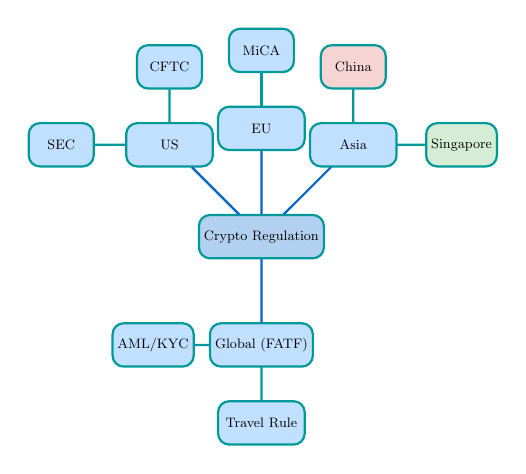
\begin{tikzpicture}[scale=0.55, transform shape,
    node distance=1.8cm,
    every node/.style={font=\small}]

% Central node
\node (reg) [blockchain, minimum width=2.5cm, fill=dfblue!30] {Crypto Regulation};

% First level
\node (us) [blockchain, above left of=reg, node distance=3cm, minimum width=2cm] {US};
\node (eu) [blockchain, above of=reg, node distance=2.5cm, minimum width=2cm] {EU};
\node (asia) [blockchain, above right of=reg, node distance=3cm, minimum width=2cm] {Asia};
\node (global) [blockchain, below of=reg, node distance=2.5cm, minimum width=2cm] {Global (FATF)};

% Second level - US
\node (sec) [blockchain, left of=us, node distance=2.5cm, minimum width=1.5cm, fill=dflightblue3] {SEC};
\node (cftc) [blockchain, above of=us, node distance=1.8cm, minimum width=1.5cm, fill=dflightblue3] {CFTC};

% Second level - EU
\node (mica) [blockchain, above of=eu, node distance=1.8cm, minimum width=1.5cm, fill=dflightblue3] {MiCA};

% Second level - Asia
\node (sg) [blockchain, right of=asia, node distance=2.5cm, minimum width=1.5cm, fill=dfgreen!20] {Singapore};
\node (cn) [blockchain, above of=asia, node distance=1.8cm, minimum width=1.5cm, fill=dfred!20] {China};

% Second level - Global
\node (travel) [blockchain, below of=global, node distance=1.8cm, minimum width=2cm, fill=dflightblue3] {Travel Rule};
\node (aml) [blockchain, left of=global, node distance=2.5cm, minimum width=1.5cm, fill=dflightblue3] {AML/KYC};

% Connections
\draw[thick, dfblue] (reg) -- (us);
\draw[thick, dfblue] (reg) -- (eu);
\draw[thick, dfblue] (reg) -- (asia);
\draw[thick, dfblue] (reg) -- (global);
\draw[thick, dfteal] (us) -- (sec);
\draw[thick, dfteal] (us) -- (cftc);
\draw[thick, dfteal] (eu) -- (mica);
\draw[thick, dfteal] (asia) -- (sg);
\draw[thick, dfteal] (asia) -- (cn);
\draw[thick, dfteal] (global) -- (travel);
\draw[thick, dfteal] (global) -- (aml);
\end{tikzpicture}
\end{center}
\end{frame}

% ==============================================================================
% SLIDE 33: Key Terms I
% ==============================================================================
\begin{frame}{Key Terms (Part 1)}
\begin{description}
\item[Howey Test] US legal test to determine if an asset is a security: investment of money in common enterprise with expectation of profits from others' efforts
\item[MiCA] Markets in Crypto-Assets---EU's comprehensive crypto regulatory framework effective 2024-2025
\item[CASP] Crypto-Asset Service Provider---licensed entity under MiCA
\item[ART] Asset-Referenced Token---stablecoin backed by multiple assets
\item[EMT] E-Money Token---stablecoin pegged 1:1 to single fiat currency
\item[VASP] Virtual Asset Service Provider---FATF term for crypto businesses
\item[Travel Rule] FATF requirement to share sender/receiver information for crypto transfers
\end{description}
\end{frame}

% ==============================================================================
% SLIDE 34: Key Terms II
% ==============================================================================
\begin{frame}{Key Terms (Part 2)}
\begin{description}
\item[Regulatory Arbitrage] Strategically choosing jurisdictions with favorable regulations
\item[Regulatory Sandbox] Controlled environment for testing innovations with relaxed rules
\item[BitLicense] New York State's comprehensive crypto business license
\item[FinCEN] Financial Crimes Enforcement Network---US AML/KYC enforcer
\item[FATF] Financial Action Task Force---sets global AML standards
\item[BSA] Bank Secrecy Act---US law requiring financial institutions to report suspicious activity
\item[MSB] Money Services Business---FinCEN registration category for crypto businesses
\item[Regulation by Enforcement] Establishing rules through lawsuits rather than clear legislation
\end{description}
\end{frame}

% ==============================================================================
% SLIDE 35: Common Misconceptions
% ==============================================================================
\begin{frame}{Common Misconceptions}
\begin{alertblock}{Misconception 1: ``Crypto is unregulated''}
\textbf{Reality:} Crypto faces extensive regulation---AML/KYC, securities laws, money transmission rules. The issue is regulatory fragmentation and unclear jurisdiction.
\end{alertblock}

\begin{alertblock}{Misconception 2: ``Decentralization means no regulation applies''}
\textbf{Reality:} Regulators can target frontends, developers, governance token holders, and infrastructure providers. Enforcement actions against DeFi are increasing.
\end{alertblock}

\begin{alertblock}{Misconception 3: ``Operating offshore avoids US rules''}
\textbf{Reality:} If you serve US customers, US law applies. Binance's \$4.3B settlement proves offshore incorporation offers limited protection.
\end{alertblock}

\begin{alertblock}{Misconception 4: ``All tokens are either securities or commodities''}
\textbf{Reality:} Classification depends on context. The same token can be a security in one sale (institutional) and not in another (exchange trading).
\end{alertblock}
\end{frame}

% ==============================================================================
% SLIDE 36: Self-Assessment Questions I
% ==============================================================================
\begin{frame}{Self-Assessment Questions (1/2)}
\textbf{Test your understanding:}
\vspace{3mm}

\textbf{Question 1:} What is the main jurisdictional difference between the SEC and CFTC in US crypto regulation?
\begin{itemize}
\item[A)] SEC regulates all cryptocurrencies while CFTC regulates only stablecoins
\item[B)] SEC has jurisdiction over securities while CFTC oversees commodities like Bitcoin
\item[C)] CFTC regulates exchanges while SEC regulates token issuers
\item[D)] There is no difference; they share identical jurisdictions
\end{itemize}

\vspace{5mm}
\textbf{Question 2:} What are the core components of AML/KYC requirements for crypto exchanges?
\begin{itemize}
\item[A)] Only requiring email addresses for all users
\item[B)] Customer identification, verification, transaction monitoring, and suspicious activity reporting
\item[C)] Collecting passport information but no ongoing monitoring
\item[D)] Anonymous trading with voluntary disclosure
\end{itemize}
\end{frame}

% ==============================================================================
% SLIDE 37: Self-Assessment Questions II
% ==============================================================================
\begin{frame}{Self-Assessment Questions (2/2)}
\textbf{Question 3:} What are common securities registration exemptions used by crypto projects?
\begin{itemize}
\item[A)] No exemptions exist; all securities must be fully registered
\item[B)] Regulation D (private placements), Regulation A+ (mini-IPO), and Regulation S (non-US offerings)
\item[C)] Projects can self-declare exemption without filing anything
\item[D)] All crypto tokens are automatically exempt as utility tokens
\end{itemize}

\vspace{5mm}
\begin{block}{Answers}
\begin{enumerate}
\item \textbf{B} -- SEC regulates securities, CFTC oversees commodities (BTC, ETH)
\item \textbf{B} -- Full AML/KYC includes ID verification, monitoring, and SARs
\item \textbf{B} -- Reg D, Reg A+, and Reg S are common exemptions (with strict requirements)
\end{enumerate}
\end{block}
\end{frame}

% ==============================================================================
% SLIDE 38: What's Next
% ==============================================================================
\begin{frame}{What's Next: Topic 5.3 -- DAO Governance}
\textbf{Preview of upcoming topic:}
\vspace{3mm}

\begin{columns}[T]
\begin{column}{0.48\textwidth}
\textbf{We will explore:}
\begin{itemize}
\item What are DAOs?
\item Token-based governance models
\item Voting mechanisms (1-token-1-vote, quadratic, conviction)
\item Governance attacks and defenses
\item Legal status of DAOs
\item Real-world DAO case studies
\end{itemize}
\end{column}
\begin{column}{0.48\textwidth}
\textbf{Key Questions:}
\begin{itemize}
\item How do decentralized organizations make decisions?
\item Can DAOs be legally recognized?
\item What happens when governance fails?
\item How do DAOs interact with regulation?
\end{itemize}
\end{column}
\end{columns}

\vspace{5mm}
\begin{block}{Connection to This Topic}
DAOs raise fundamental regulatory questions: If a DAO controls a protocol, who is liable? Can governance token holders be regulated? These questions build directly on our regulatory analysis.
\end{block}
\end{frame}

% ==============================================================================
% SLIDE 39: Resources
% ==============================================================================
\begin{frame}{Resources for Further Learning}
\textbf{Primary Sources:}
\begin{itemize}
\item MiCA Regulation: \url{eur-lex.europa.eu} (search ``MiCA'')
\item SEC Crypto Guidance: \url{sec.gov/spotlight/cybersecurity}
\item FATF Virtual Assets: \url{fatf-gafi.org/en/topics/virtual-assets.html}
\item FinCEN Guidance: \url{fincen.gov/resources/statutes-and-regulations}
\end{itemize}

\vspace{3mm}
\textbf{Recommended Reading:}
\begin{itemize}
\item ``Cryptoassets: Legal, Regulatory, and Monetary Perspectives'' -- Chris Brummer
\item SEC DAO Report (2017) -- The DAO investigation report
\item Howey Test Case: SEC v. W.J. Howey Co., 328 U.S. 293 (1946)
\end{itemize}

\vspace{3mm}
\textbf{Tools:}
\begin{itemize}
\item Chainalysis regulatory compliance reports
\item Elliptic compliance resources
\end{itemize}
\end{frame}

% ==============================================================================
% SLIDE 40: Questions Closing Slide
% ==============================================================================
\begin{frame}[plain]
\begin{center}
\vspace{1cm}
{\Huge \textbf{Questions?}}

\vspace{1cm}
{\Large Topic 5.2: Regulatory Landscapes}

\vspace{0.5cm}
{\large Global Approaches to Digital Finance Regulation}

\vspace{1.5cm}
\textbf{Joerg Osterrieder}\\
Digital Finance\\
2025

\vspace{1cm}
{\small Next: Topic 5.3 -- DAO Governance}
\end{center}
\end{frame}

\end{document}
